\documentclass[]{beamer}

\usepackage{beamerthemesplit}
\usepackage{amsmath}
\usepackage{algorithm}
\usepackage{algpseudocode}
\usepackage{enumerate}
\usepackage{color}
\usepackage{graphicx}
\usepackage{float}
\usepackage{pgfpages}
\usepackage{multimedia}

\setbeameroption{hide notes}
%\setbeameroption{show notes}
%\setbeameroption{show notes on second screen=right}
%\useoutertheme{infolines}
\usetheme{Warsaw}

\newcommand{\mb}[1]{\mathbf{#1}}


\title{Review on Boosting Algorithm}
\author{Quoc Khanh \textsc{DO}\\Tuan Hung \textsc{VU}\\ - Advisor: Dr.~Stéphan \textsc{Clémençon}}
\date{\today}

\AtBeginSection[]
{
   \begin{frame}
       \frametitle{Outline}
       \tableofcontents[currentsection]
   \end{frame}
}

\begin{document}

\frame{\titlepage}
\section*{Outline}
\begin{frame}
	\frametitle{Outline}
	\tableofcontents[currentsections]
\end{frame}


%%%%%%%Introduction%%%%%%%%%%%%%%%%%%%
%%%%%%%%%%%%%%%%%%%%%%%%%%%%%%%%%%%%%%%%%%%%%%%%%%%%%%%%%%%%%%%%%%%%%%%%%%%%%%%%%%%%%%%%%%%%%%%%
\section{Experiment}
%===============================================%
\subsection{Binary Classification Boosting Algorithm}
\begin{frame}
	\frametitle{Experiment 1}
	\begin{itemize}
		\item Goal: Compare binary classification boosting algorithms:
			\begin{itemize}
				\item Least-Square TreeBoost
				\item LAD TreeBoost
				\item M-TreeBoost
				\item Gentle AdaBoost
				\item Logit Boost
				\item L2-TreeBoost
			\end{itemize}

		\item Simulated dataset:
			\begin{itemize}
				\item 500 samples: 2-dimensional explanatory vectors
				\item Label = $\{-1, 1\}$
				\item Number of iteration for learning each algorithm: 100
				\item Number of Monte Carlo iterations: 100
			\end{itemize}
	\end{itemize}
\end{frame}
%===============================================%
\begin{frame}
	\frametitle{Result}
	\begin{figure}
		\caption{Comparison of Boosting Algorithms with Binary Classification}
		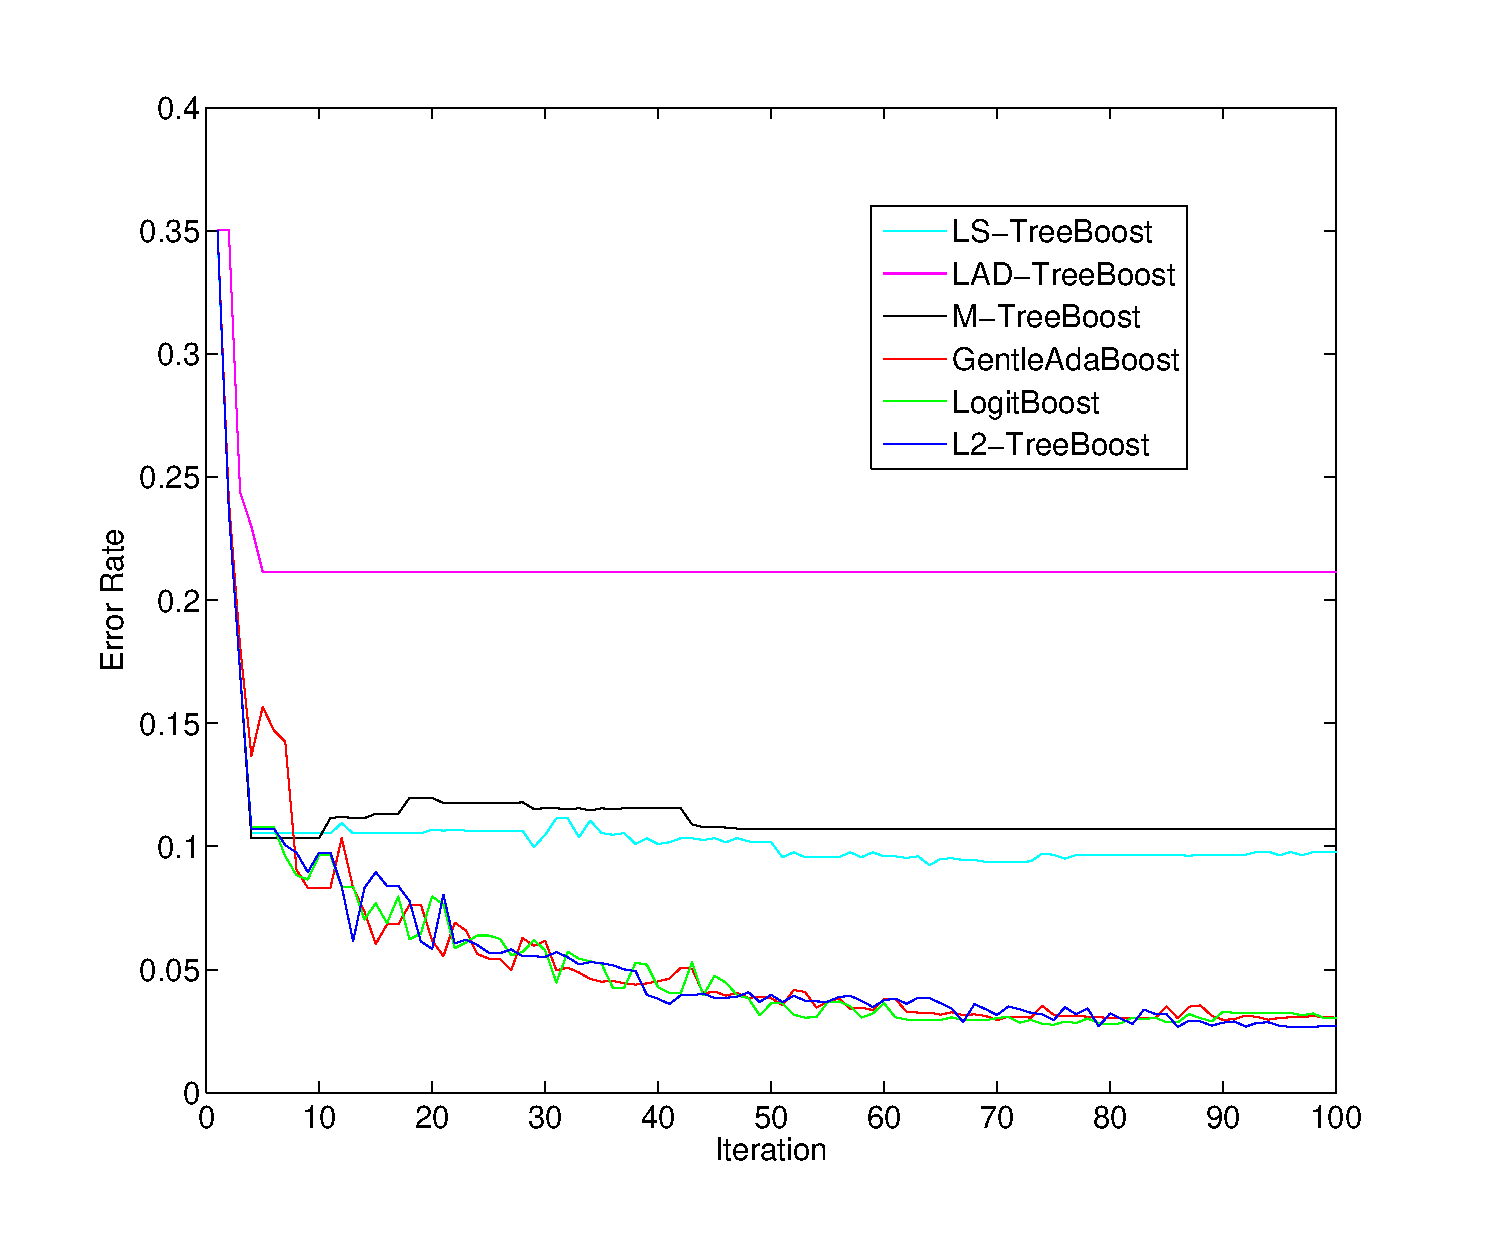
\includegraphics[width = 0.7\textwidth]{Figures/bin_class_comparison.eps}
	\end{figure}
\end{frame}
%===============================================%
\begin{frame}
	\frametitle{Result}
	\begin{figure}
		\caption{Comparison of Boosting Algorithms with Binary Classification with 5\% Noise}
		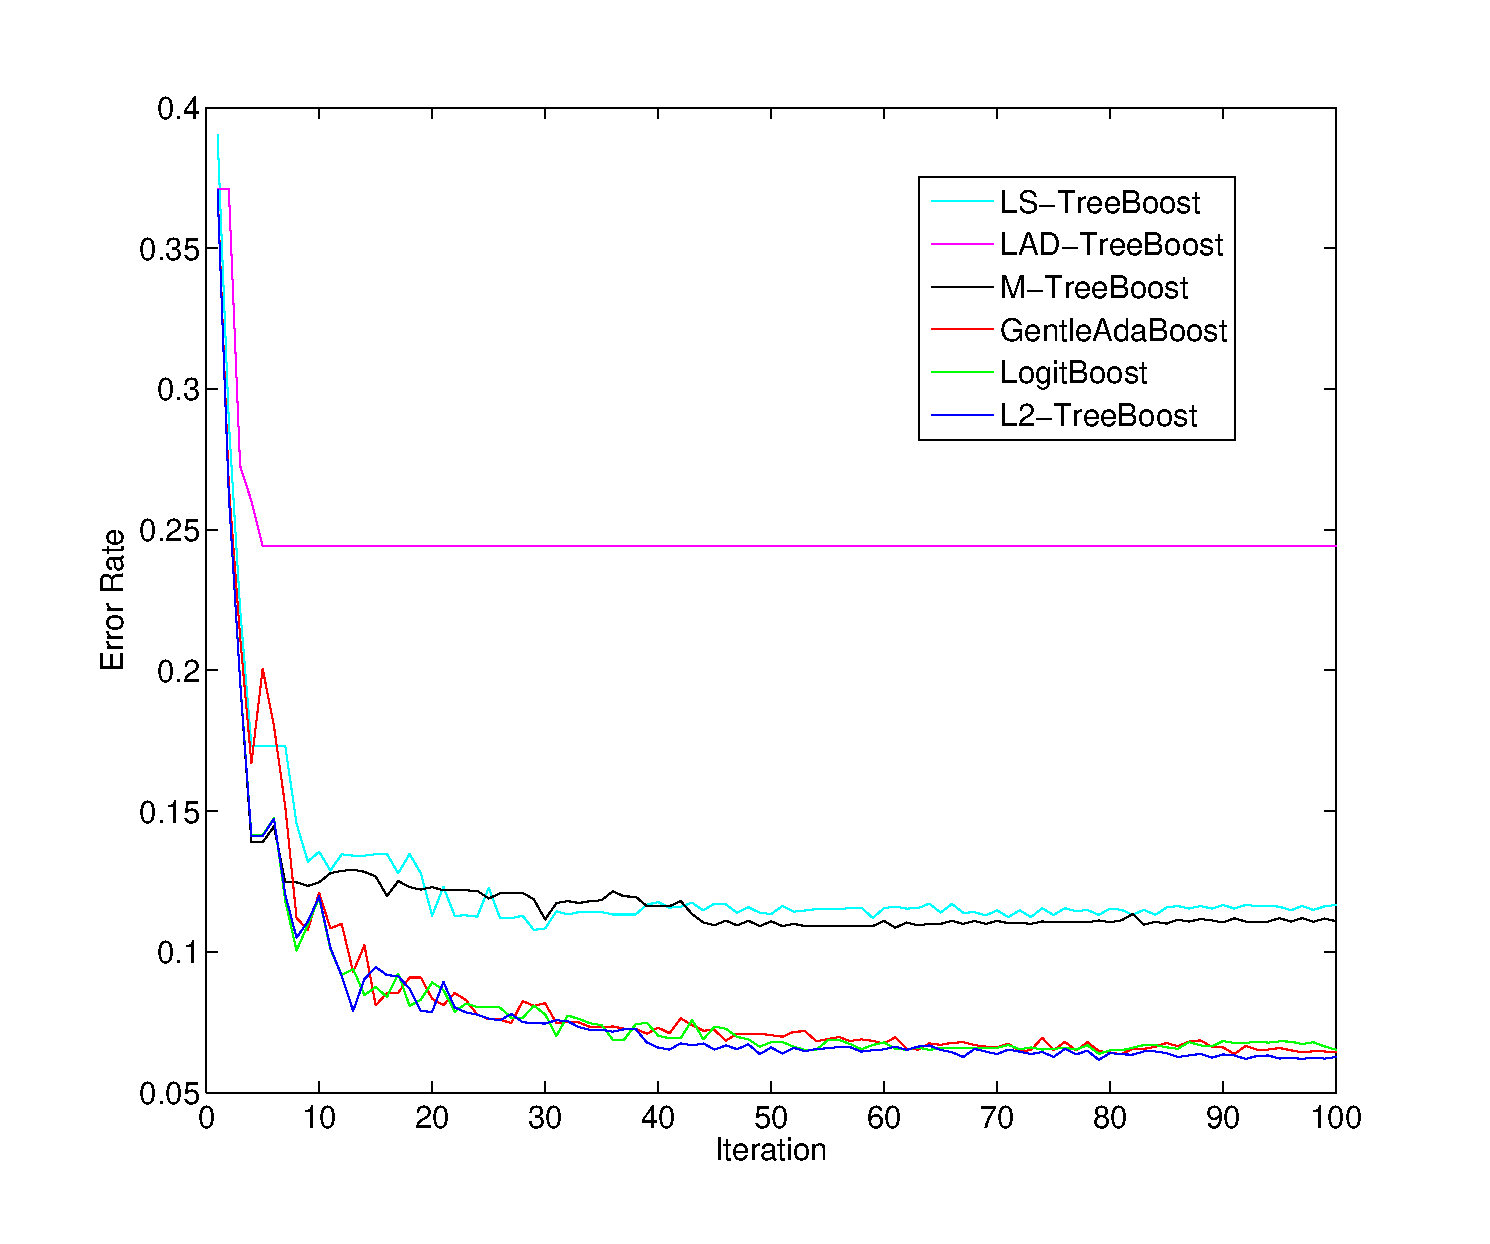
\includegraphics[width = 0.7\textwidth]{Figures/bin_class_comparison_noise_5per.eps}
	\end{figure}
\end{frame}
%===============================================%
\begin{frame}
	\frametitle{Result}
	\begin{figure}
		\caption{Comparison of Boosting Algorithms with Binary Classification with 10\% Noise}
		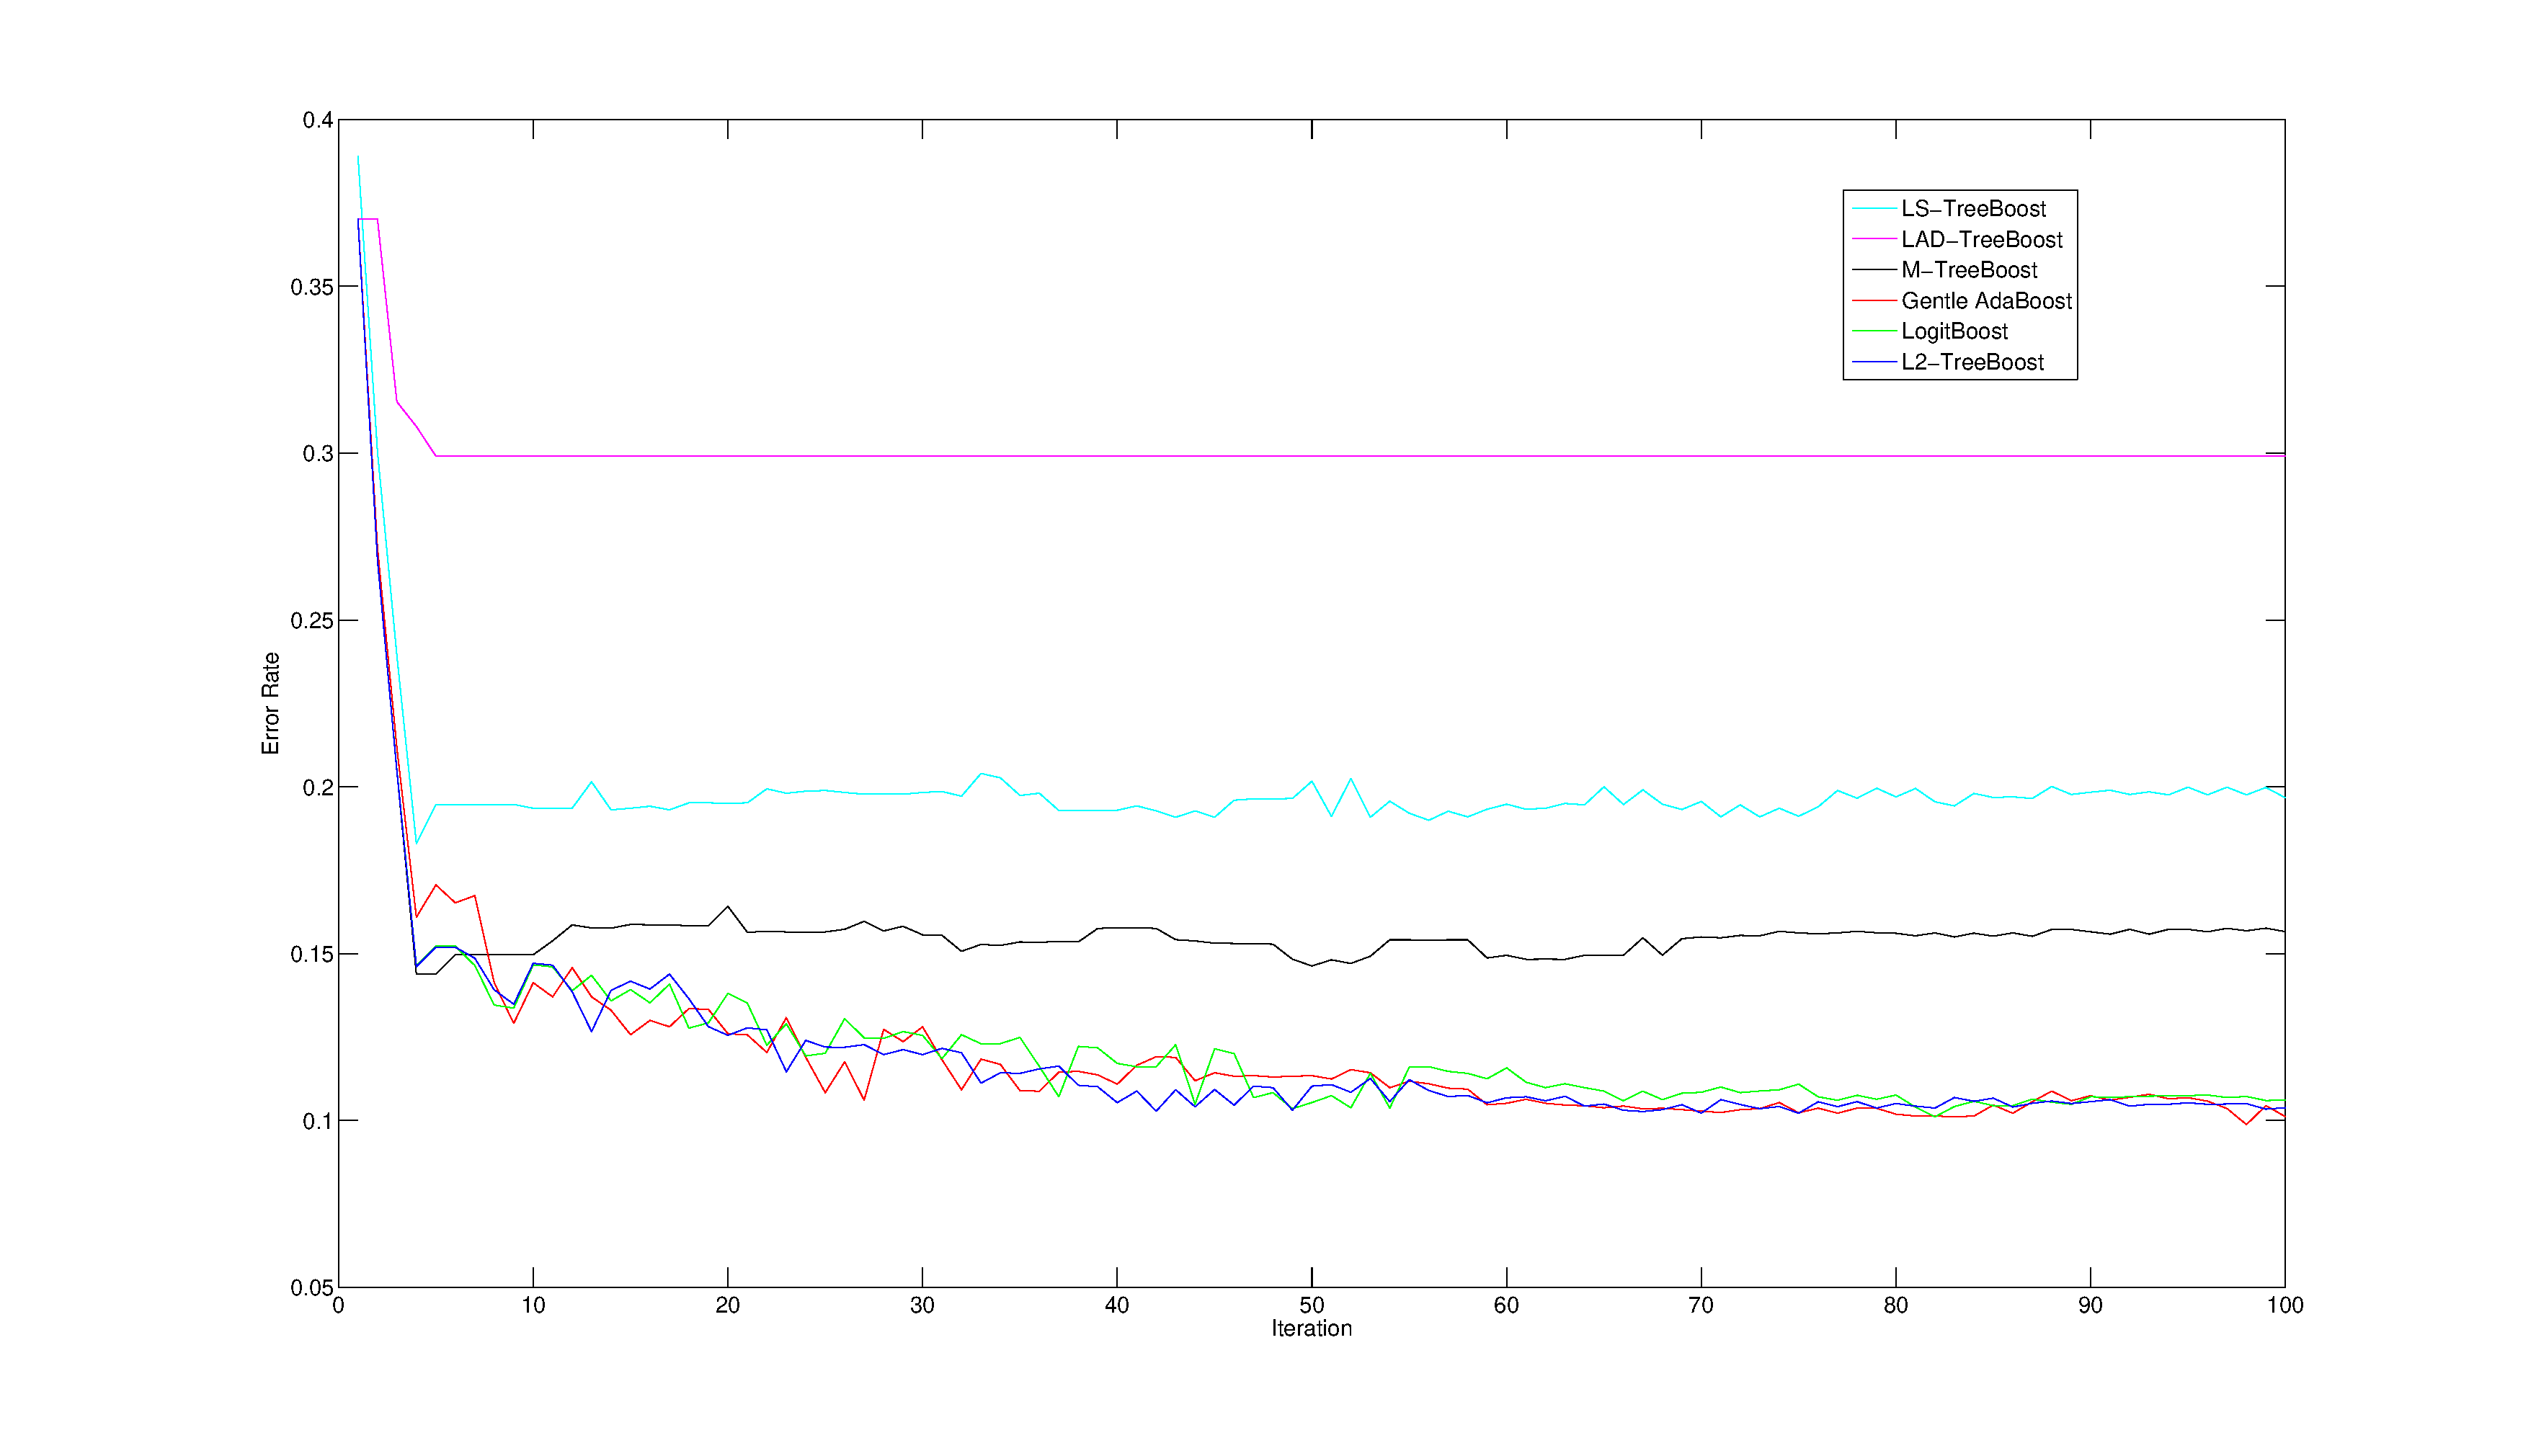
\includegraphics[width = 0.7\textwidth]{Figures/bin_class_comparison_noise_10per.eps}
	\end{figure}
\end{frame}
%===============================================%
\begin{frame}
	\frametitle{Experiment 2}
	\begin{itemize}
		\item Goal: Compare binary classification boosting algorithms:
			\begin{itemize}
				\item Least-Square TreeBoost
				\item LAD TreeBoost
				\item M-TreeBoost
				\item Gentle AdaBoost
				\item Logit Boost
				\item L2-TreeBoost
			\end{itemize}

		\item Real dataset: UCI Wisconsin Breast Cancer Dataset
			\begin{itemize}
				\item 683 samples: 9-dimensional explanatory vectors
				\item Label = $\{2, 4\}$
				\item 5 fold cross validation
			\end{itemize}
	\end{itemize}
\end{frame}
%===============================================%
\begin{frame}
	\frametitle{Result}
	\begin{figure}
		\centering
		\caption{Comparison of Boosting Algorithms with UCI Wisconsin Breast Cancer Dataset}
		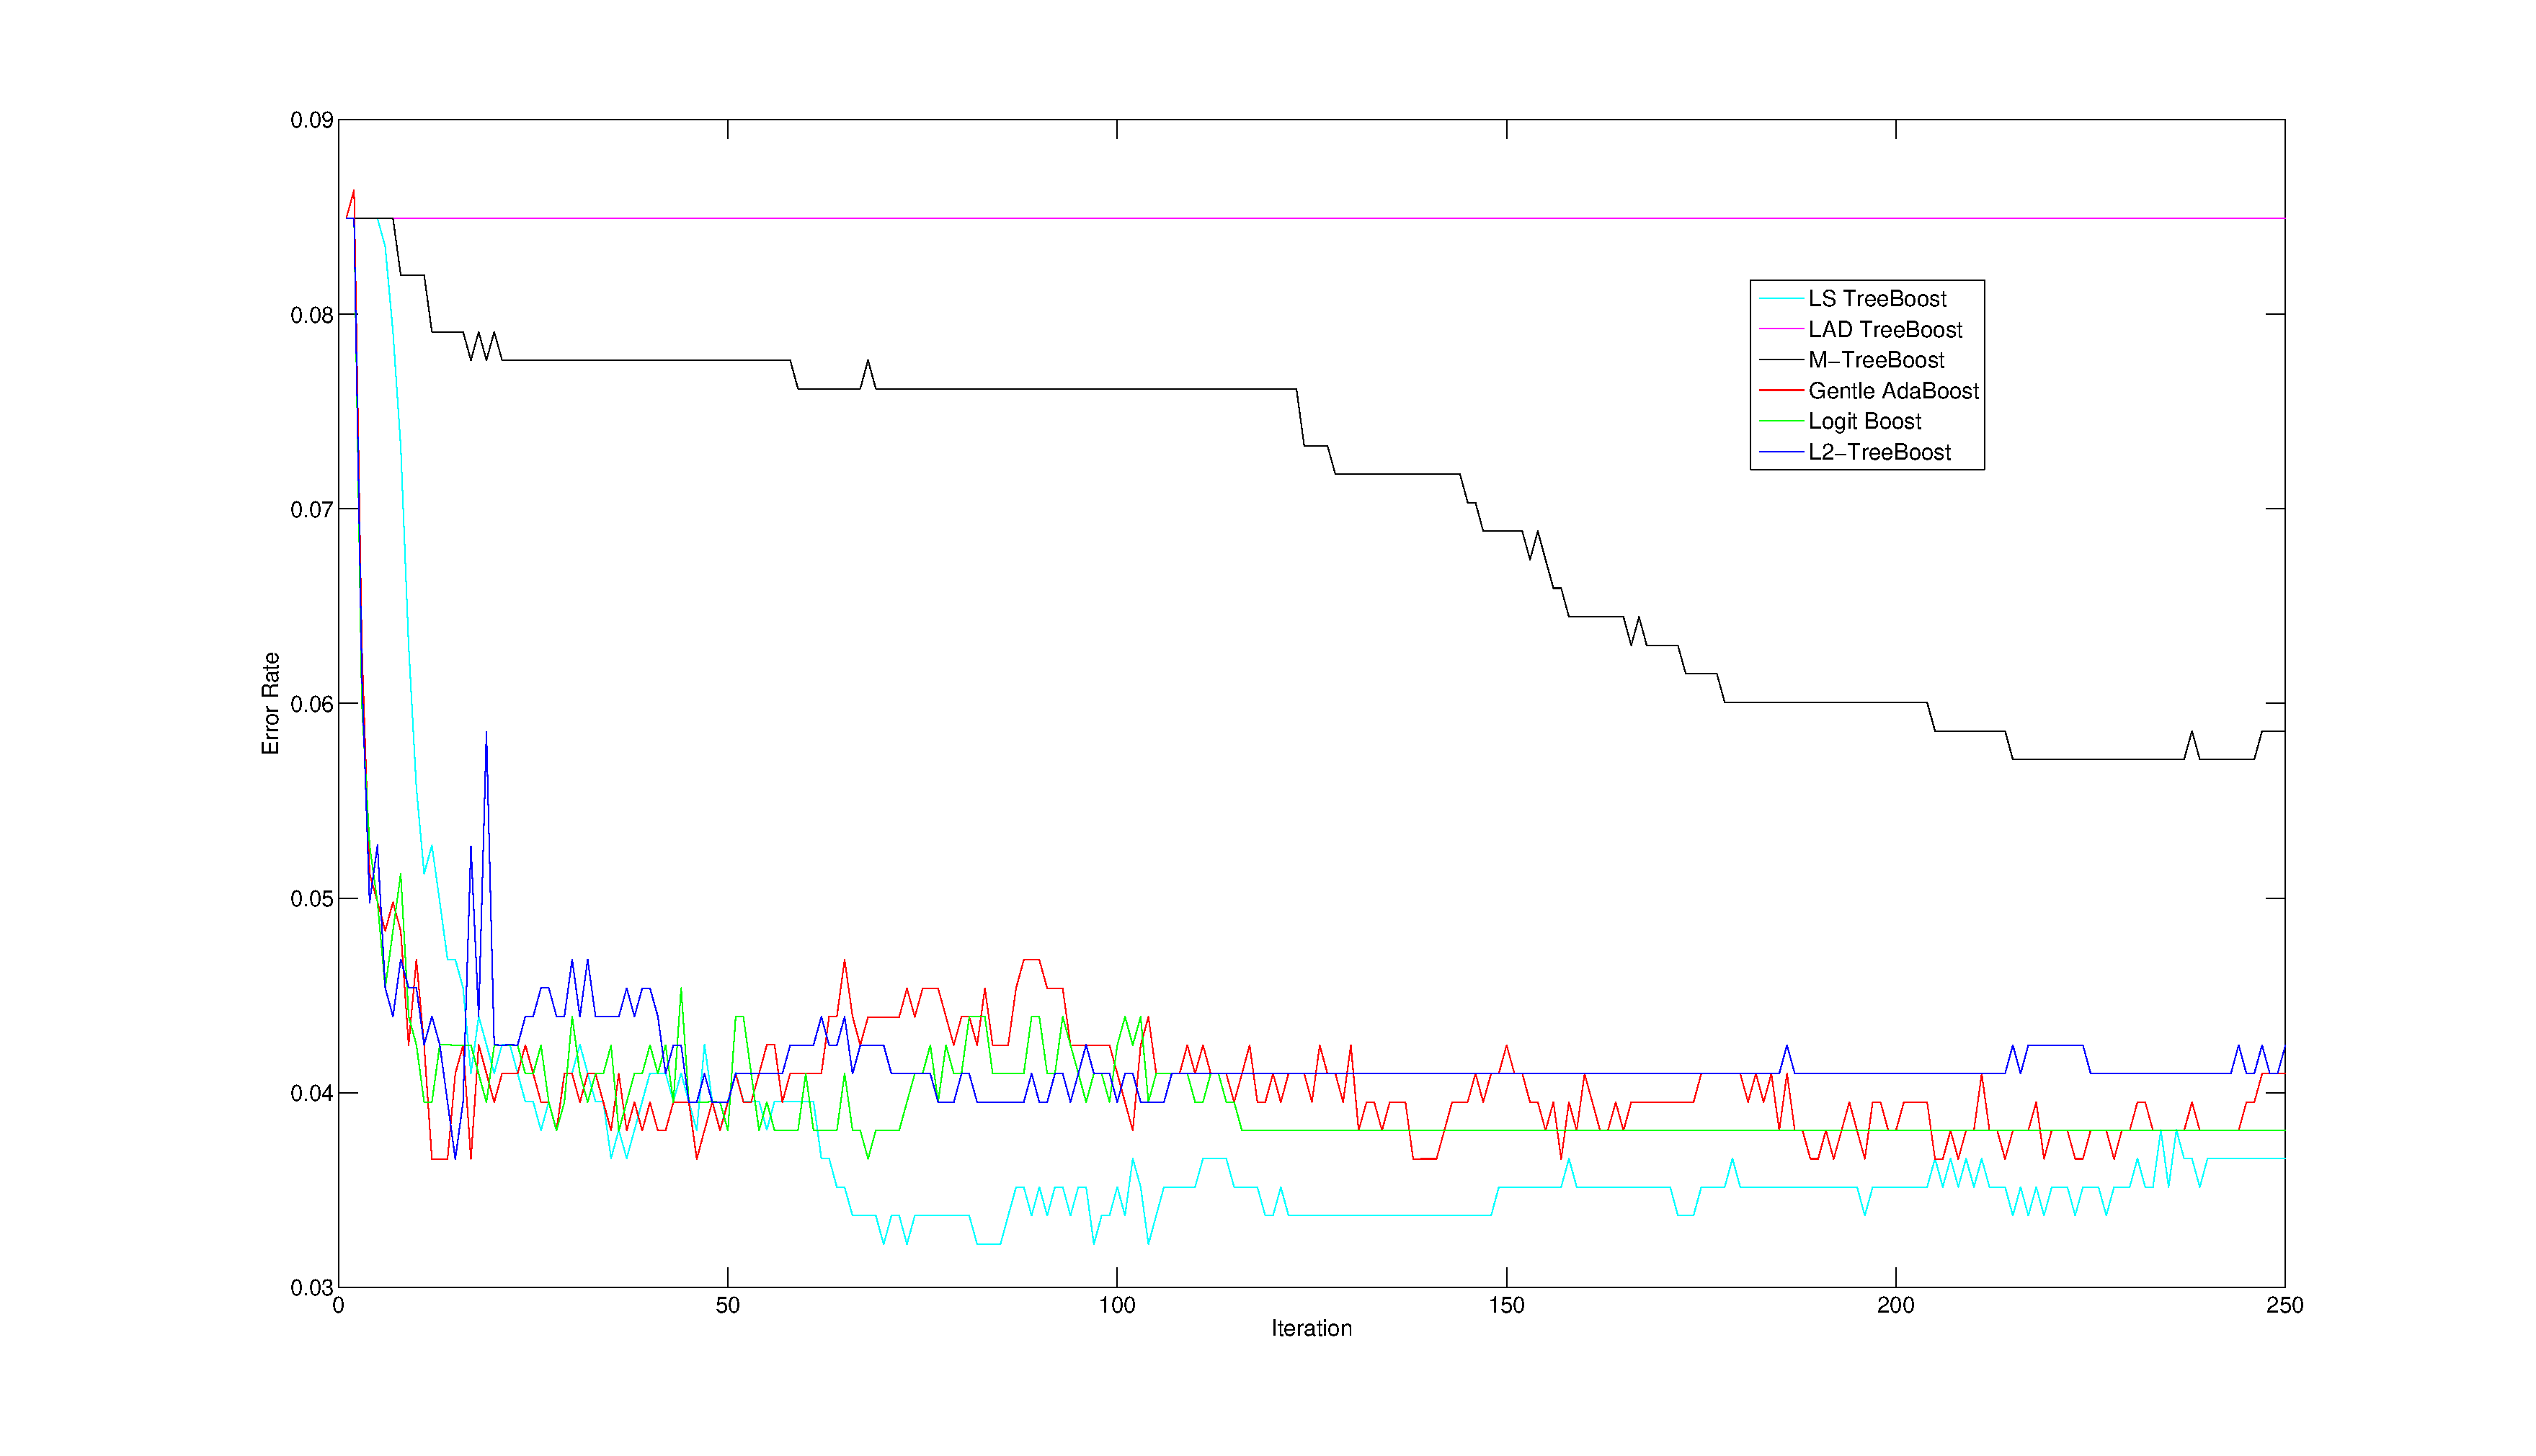
\includegraphics[width = 0.7\textwidth]{Figures/wbc.eps}
	\end{figure}
\end{frame}

%===============================================%
\subsection{Multi-class Classification Boosting Algorithm}
%===============================================%
\begin{frame}
	\frametitle{Experiment}
	\begin{itemize}
		\item Goal: Compare multi-class classification boosting algorithms:
			\begin{itemize}
				\item AdaBoost MH
				\item Logit Boost for J class
				\item Multiclass TreeBoost
			\end{itemize}

		\item Real dataset: UCI Wine quality
			\begin{itemize}
				\item 1599 samples: 11-dimensional explanatory vectors
				\item Label = 0:10
				\item 5 fold cross validation
			\end{itemize}
	\end{itemize}
\end{frame}
%===============================================%
\begin{frame}
	\frametitle{Result}
	\begin{figure}[H]
		\centering
		\caption{Comparison of Multi-class Boosting Algorithms with UCI Wine Quality Dataset}
		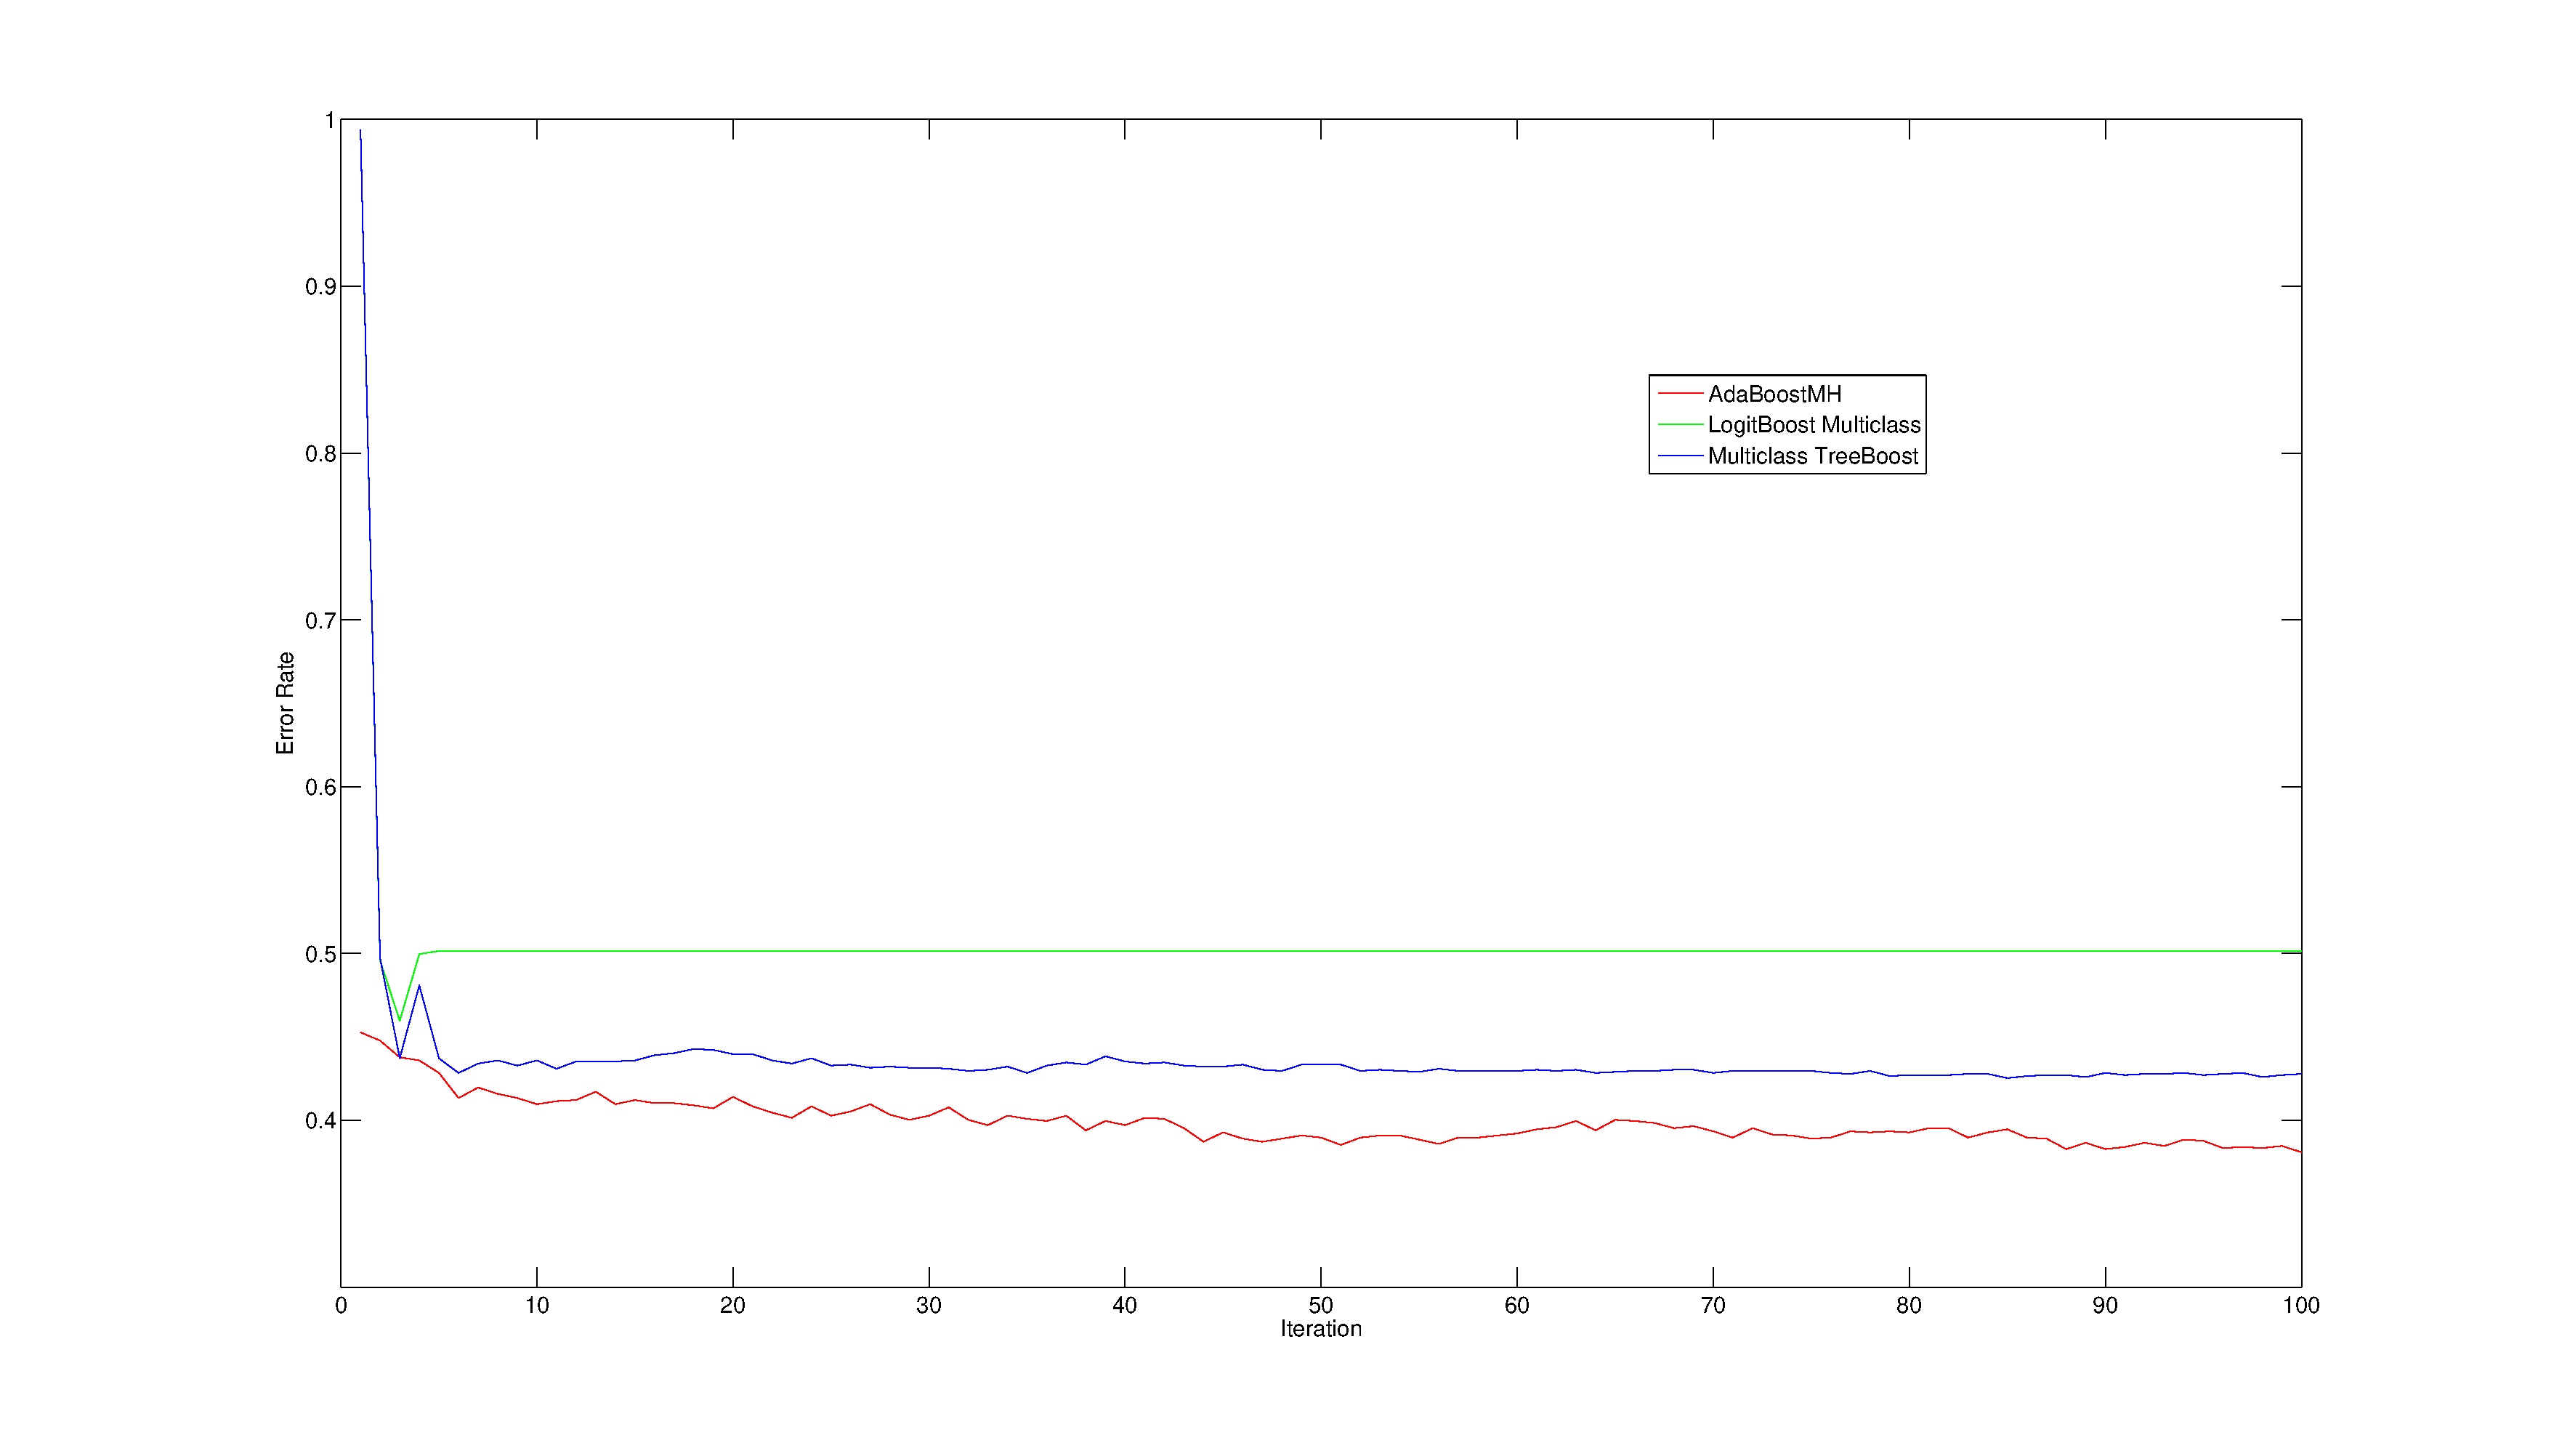
\includegraphics[width = 0.7\textwidth]{Figures/wine_quality.eps}
	\end{figure}
\end{frame}



%%%%%%%References%%%%%%%%%%%%%%%%%%%%%%%%%%%%%%%%%%%%%%%%%%%%%%%%%%%%%%%%%%%%%%%%%%%%%%%%%%%%%%%%%%%%%%%%%%%%%%%%%%%%%%%%%%%%%%%%%%%
\section*{References}
\frame[allowframebreaks]{
	\frametitle{References}
	\bibliographystyle{acm}
	\bibliography{mypapers}
}

\end{document}